\section{Potentiale}\label{sec:Potentiale}

Eine Schwierigkeit bei der Analyse von Spielen bildet der Umstand, dass jeder Spieler eine eigene Kostenfunktion und damit ein eigenes Optimierungsziel hat. Möchte man also beispielsweise Gleichgewichtspunkte finden, so muss man alle diese Funktionen gleichzeitig (lokal) optimieren. Diese Aufgabe wird wesentlich einfacher, wenn das Spiel eine sogenannte \emph{Potentialfunktion} besitzt. Das ist eine Funktion auf dem Strategieraum des Spieles, die ein alternatives Koordinationsspiel darauf definiert, welches gewisse Eigenschaften mit dem ursprünglichen Spiel teilt (etwa die Lage der Gleichgewichtspunkte).

In diesem Kapitel werden wir einige Varianten von Potentialfunktionen kennenlernen und feststellen, welche Spiele diese jeweils besitzen. In \Cref{sec:Morphismen} werden wir dann die Beziehung zwischen Ausgangsspiel und dem von einer Potentialfunktion darauf beschriebenen Koordinationsspiel durch Morphismen zwischen den beiden Spielen formalisieren und dadurch zeigen, welche Eigenschaften beim Wechsel zwischen den beiden Spielen erhalten bleiben.

\subsection{Definitionen}

Zunächst definieren wir eine Auswahl verschiedener Arten von Potentialfunktionen:

\begin{defn}
	Zu einem Spiel $\Gamma = (I, X, (c_i))$ heißt eine Funktion $P: X \to \IR$
	\begin{itemize}
		\item \emph{verallgemeinertes Nash-Potential}, wenn jedes Minimum von $P$ ein Nash-Gleichgewicht in $\Gamma$ ist, d.h. für alle $x \in X$ gilt:
			\[P(x) = \min_{\hat{x} \in X}P(\hat{x}) \implies \forall i \in I, \hat{x}_i \in X_i: c_i(x) \leq c_i(x \mid \hat{x}_i) \]
		\item \emph{Nash-Potential}, wenn jedes Minimum von $P$ ein Nash-Gleichgewicht in $\Gamma$ ist und umgekehrt, d.h. für alle $x \in X$ gilt:
			\[P(x) = \min_{\hat{x} \in X}P(\hat{x}) \iff \forall i \in I, \hat{x}_i \in X_i: c_i(x) \leq c_i(x \mid \hat{x}_i) \]
		\item \emph{lokales Nash-Potential}, wenn jedes \glqq lokale\grqq{} Minimum von $P$ ein Nash-Gleichgewicht in $\Gamma$ ist und umgekehrt, d.h. für alle $x \in X$ gilt:
			\[\forall i \in I, \hat{x}_i \in X_i: P(x) \leq P(x \mid \hat{x}_i) \iff \forall i \in I, \hat{x}_i \in X_i: c_i(x) \leq c_i(x \mid \hat{x}_i) \]
		\item \emph{Beste-Antwort-Potential}, wenn für jeden Spieler $i$ und alle Strategieprofile $x \in X$ gilt:
			\[\arg\min_{\hat{x}_i \in X_i}c_i(x \mid \hat{x}_i) = \arg \min_{\hat{x}_i \in X_i} P(x \mid \hat{x}_i)\]
		\item \emph{verallgemeinertes ordinales Potential}, wenn für jeden Spieler $i$ und alle Strategieprofile $x \in X$ sowie $\hat{x}_i \in X_i$ gilt:
			\[c_i(x) > c_i(x \mid \hat{x}_i) \implies P(x) > P(x \mid \hat{x}_i)\]
		\item \emph{ordinales Potential}, wenn für jeden Spieler $i$ und alle Strategieprofile $x \in X$ sowie $\hat{x}_i \in X_i$ gilt:
			\[c_i(x) > c_i(x \mid \hat{x}_i) \iff P(x) > P(x \mid \hat{x}_i)\]
		\item \emph{skaliertes Potential}, wenn es streng monotone Funktionen $f_i: \IR \to \IR$ gibt, sodass für jeden Spieler $i$ und alle Strategieprofile $x \in X$ sowie $\hat{x}_i \in X_i$ gilt:
			\[c_i(x) - c_i(x \mid \hat{x}_i) = f_i(P(x)) - f_i(P(x \mid \hat{x}_i))\]
		\item \emph{gewichtetes Potential}, wenn es einen Gewichtsvektor $(w_i)_{i\in I} \in \IR_{>0}^I$ gibt, sodass für jeden Spieler $i$ und alle Strategieprofile $x \in X$ sowie $\hat{x}_i \in X_i$ gilt:
			\[c_i(x) - c_i(x \mid \hat{x}_i) = w_i\cdot(P(x) - P(x \mid \hat{x}_i))\]
		\item \emph{exaktes Potential}, wenn für jeden Spieler $i$ und alle Strategieprofile $x \in X$ sowie $\hat{x}_i \in X_i$ gilt:
			\[c_i(x) - c_i(x \mid \hat{x}_i) = P(x) - P(x \mid \hat{x}_i)\]
	\end{itemize}
\end{defn}

Exakte, gewichtete, ordinale und verallgemeinerte ordinale Potentiale wurden erstmals in \cite{MonShap} definiert, beste Antwort-Potentiale erstmals in \cite{BestRespPot}. Die Begriffe verallgemeinertes und lokales Nash-Potential dürften für die Anwendung eher weniger interessant sein, sondern sollen vor allem das grundlegende Konzept eines Potentials formalisieren und umfassen daher auch (fast) alle anderen Potentiale. Die Beziehungen zwischen den verschiedenen Potentialbegriffen werden in dem an \cite[Abbildung 1]{BestRespPot} angelehnten Euler-Diagramm (\Cref{diag:Potentiale}) dargestellt.

\begin{figure}[h]\centering
	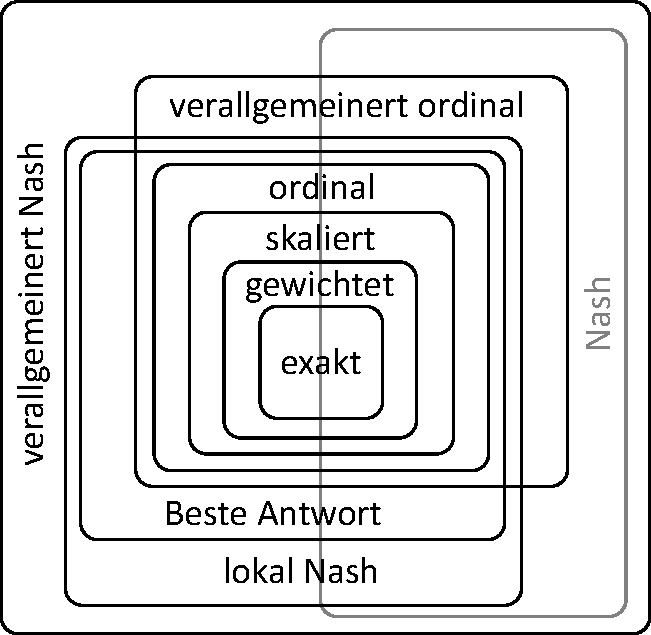
\includegraphics[width=.4\textwidth]{../Bilder/EulerDiagPotentiale.pdf}
	\caption{Beziehungen zwischen den einzelnen Potentialbegriffen}\label{diag:Potentiale}
\end{figure}

\begin{bsp}
	Jedes Koordinationsspiel besitzt ein exaktes Potential (nämlich die gemeinsame Kostenfunktion). Entsprechend besitzt jedes skalierte Koordinationsspiel ein skaliertes Potential und jedes Dummyspiel ein exaktes Potential (die konstante $0$-Funktion).
\end{bsp}

\subsection{Anschauung}

Verallgemeinerte Nash-Potentiale (und damit alle oben beschriebenen Potentiale) formalisieren die Idee, ein Spiel durch irgendein anderes mit einer einzigen Funktion beschriebenes Optimierungsproblem zu ersetzen, dessen Optima Nash-Gleichgewichte im ursprünglichen Spiel sind. Im Falle eines Nash-Potentials entsprechen diese Optima sogar \emph{allen} Nash-Gleichgewichten. Findet man nun ein solches Optimierungsproblem und kann von diesem zeigen, dass es immer ein Optimum besitzt (etwa weil es durch eine stetige Funktion beschrieben wird und der Strategieraum kompakt ist), so zeigt dies, dass das ursprüngliche Spiel mindestens ein Nash-Gleichgewicht besitzt. Außerdem lässt sich dieses durch Lösen des Optimierungsproblems bestimmen.

Versteht man zu einem gegebenen Strategieprofil $x \in X$ dessen \emph{Nachbarschaft} als die Menge aller durch höchstens einen Schritt erreichbarer Strategieprofile, d.h. die Menge $\set{(x \mid \hat{x}_i) | i \in I, \hat{x}_i \in X_i}$, so nennen wir $x$ ein \emph{lokales Minimum} einer Funktion $P: X \to \IR$, wenn es ein Minimum innerhalb seiner Nachbarschaft ist. Ein lokales Nash-Potential beschreibt damit ein Optimierungsproblem, dessen \emph{lokale} Minima den Nash-Gleichgewichten des Ausgangsspiels entsprechen.

Die Nachbarschaft eines Strategieprofils $x$ besteht nun gerade aus den Profilen, die man mit $x$ vergleichen muss, um festzustellen, ob es sich bei $x$ um ein Nash-Gleichgewicht handelt. Hat man also ein Spiel $\Gamma = (I, X, (c_i))$ mit einem lokalen Nash-Potential $P$, so induziert dieses ein Koordinationsspiel $\Kappa \coloneqq (I, X, (P))$ auf dem selben Strategieraum, dessen Nash-Gleichgewichte gerade mit denen des Ausgangsspiels $\Gamma$ übereinstimmen.

Weitere Spezialisierungen des Potentialbegriffs führen dann zu induzierten Koordinationsspielen, welche noch mehr Eigenschaften des Ausgansspiels übernehmen: So hat das durch ein Beste-Antwort-Potential beschriebene Spiel etwa die gleichen Beste-Antwort-Pfade und eignet sich daher beispielsweise zur Analyse von Beste-Antwort-Dynamiken (vgl. \Cref{sec:Auslastungsspiele:BADynamiken}). Durch ein ordinales Potential erhält man ein Spiel, welches auch die gleichen Verbesserungs- und Nichtverschlechterungspfade besitzt. Bei einem verallgemeinerten ordinalen Potential bleiben diese hingegen jeweils nur in eine Richtung erhalten: Ein Verbesserungspfad im Ausgangsspiel ist auch einer im Koordinationsspiel und ein Nichtverschlechterungspfad im Koordinationsspiel entspricht einem solchen im ursprünglichen Spiel (vgl. \Cref{prop:ordPotVerbpfad} bzw. \Cref{prop:NVReflVerbErh}).

Für skalierte, gewichtete und exakte Potentiale gibt es eine noch anschaulichere Betrachtungsweise für den Fall (endlicher) 2-Personenspiele. Statt als Matrix kann man deren Strategieraum auch als Gitternetz in der Ebene auffassen, wobei jede Strategie von Spieler 1 einer waagerechten und jede Strategie von Spieler 2 einer senkrechten Gitterlinie entspricht. Kreuzungspunkte von zwei Geraden entsprechen dann vollständigen Strategieprofilen und Kostenfunktionen (ebenso wie Potentiale) sind \glqq Reliefkarten\grqq{}, deren Höhe den jeweiligen Kosten entspricht. 

\begin{figure}[ht]\centering
	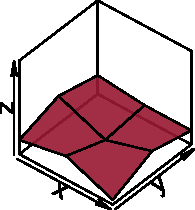
\includegraphics[width=.3\textwidth]{../Bilder/exaktesPotentialSp1.pdf}
	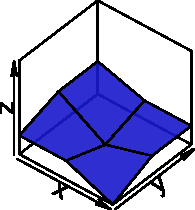
\includegraphics[width=.3\textwidth]{../Bilder/exaktesPotentialSp2.pdf}
	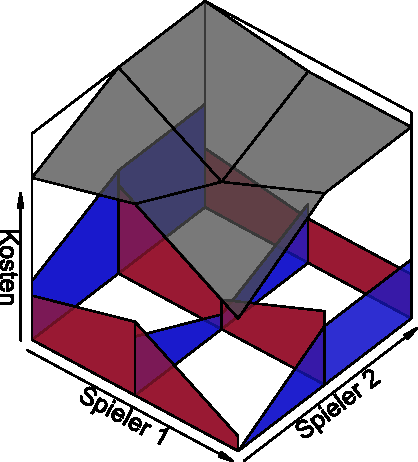
\includegraphics[width=.3\textwidth]{../Bilder/exaktesPotential.pdf}
	\caption{Ein 2-Personenspiel mit exaktem Potential (grau): Spieler 1: rot, Spieler 2: blau}
\end{figure}

Ein Potential ist in diesem Bild eine gemeinsame Reliefkarte für beide Spieler, die - im Falle eines exakten Potentials - \glqq scheibenweise\grqq{} bis auf eine additive Konstante mit der eigentlichen Kostenfunktion übereinstimmt. Anders formuliert: Wird die Strategie eines Spielers festgehalten, so kann der andere Spieler seine Kostenveränderungen bei der Wahl der verschiedenen ihm zur Verfügung stehenden Strategien auch anhand der Potentialfunktion ablesen. 

Geht man nun über zu einem skalierten Potential, so lesen die beiden Spieler das Potential sozusagen in verschiedenen Einheiten ab (müssen das Potential also erst noch passend skalieren um ihre tatsächliche Veränderung zu bekommen). Sind die Skalierungsfunktionen linear (das Potential damit ein gewichtetes), dann sind die verschiedenen Einheiten proportional zueinander.


\subsection{Eigenschaften der Potentiale}

Wir wollen hier noch einige Eigenschaften der verschiedenen Potentiale zusammenfassen - beweisen werden wir sie aber erst später.

\begin{satz}\label{satz:ZusammenaengePotentiale}
	Es gelten die in \Cref{diag:Potentiale} dargestellten Zusammenhänge zwischen den verschiedenen Potentialen.
\end{satz}

Die Zusammenhänge lassen sich alle leicht direkt beweisen. Wir werden diese Beweise hier allerdings nicht führen, da sich die Aussagen auch aus den allgemeineren Sätzen über die entsprechenden Morphismen ergeben, die wir in \Cref{sec:Morphismen} definieren werden (die Beweise finden sich dann in \Cref{sec:Morphismen:Potentialsaetze}). Dass die unterschiedlichen Potentiale tatsächlich echt verschiedene Klassen von Spielen beschreiben, zeigen die folgenden Beispiele: 

\begin{bsp}\label{bsp:PotentialInklusionen}
	Es sei jeweils $\gamma \coloneqq ((t,l), (t,r), (b,r), (b,l))$ der $4$-Zykel, der den Strategieraum im Uhrzeigersinn durchläuft. Zum Beweis, dass ein Spiel ein bestimmtes Potential nicht besitzen kann, verwenden wir zum Teil bereits die entsprechenden Charakterisierungen aus \Cref{sec:Potentiale:Charakterisierungen}.
	\begin{itemize}
		\item $\Gamma_1$ besitzt ein gewichtetes, aber kein exaktes Potential:
			\begin{center}
				$\Gamma_1:$ \quad
				\begin{tabular}{c||c|c}
					& l 		& r 		\\\hline\hline
					t	& $(0,0)$	& $(0,0)$	\\\hline
					b	& $(0,0)$	& $(1,2)$ 
				\end{tabular}\hspace{5em}
				$P_1:$ \quad
				\begin{tabular}{c||c|c}
					& l 		& r 		\\\hline\hline
					t	& $0$	& $0$	\\\hline
					b	& $0$	& $1$ 
				\end{tabular}
			\end{center}
			$P_1$ ist ein gewichtetes Potential (mit Gewichtsvektor $(1,2)$), aber $\Gamma_1$ kann nach \Cref{satz:CharExPot} kein exaktes Potential besitzen, da die Pfadänderung $\PfadAend(\gamma) = 0 + 1 - 2 + 0 \neq 0$ ist.
		
		\item $\Gamma_2$ besitzt ein skaliertes, aber kein gewichtetes Potential:
			\begin{center}
				$\Gamma_2:$ \quad
				\begin{tabular}{c||c|c}
					& l 		& r 		\\\hline\hline
					t	& $(0,0)$	& $(0,1)$	\\\hline
					b	& $(1,0)$	& $(2,1)$ 
				\end{tabular}\hspace{5em}
				$P_2:$ \quad
				\begin{tabular}{c||c|c}
					& l 		& r 		\\\hline\hline
					t	& $0$	& $1$	\\\hline
					b	& $1$	& $2$ 
				\end{tabular}
			\end{center}
			$P_2$ ist ein skaliertes Potential (mit den Skalierungsfunktionen $f_1(0) \coloneqq 0, f_1(1) = 1, f_1(2) = 3$ und $f_2 \coloneqq \id$). $\Gamma_2$ kann aber kein gewichtetes Potential besitzen. Denn gäbe es ein solches und wäre $w = (w_1, w_2)$ der zugehörige Gewichtsvektor, so würde nach \Cref{satz:CharGewPot} für die gewichtete Pfadänderung gelten:
				\[0 = \PfadAend_w(\gamma) = w_2(1-0) + w_1(2-0) + w_2(0-1) + w_1(0-1) = w_1 \]
			Das wäre jedoch ein Widerspruch dazu, dass Gewichtsvektoren positiv sein müssen.
			
		\item $\Gamma_3$ besitzt ein ordinales, aber kein skaliertes Potential:
			\begin{center}
				$\Gamma_3:$ \quad
				\begin{tabular}{c||c|c}
					& l 		& r 		\\\hline\hline
					t	& $(0,0)$	& $(0,0)$	\\\hline
					b	& $(1,0)$	& $(2,0)$ 
				\end{tabular}\hspace{5em}
				$P_3:$ \quad
				\begin{tabular}{c||c|c}
					& l 		& r 		\\\hline\hline
					t	& $0$	& $0$	\\\hline
					b	& $1$	& $1$ 
				\end{tabular}
			\end{center}
			$P_3$ ist ein ordinales Potential, $\Gamma_3$ besitzt aber kein skaliertes Potential. Denn wäre $P$ ein solches skaliertes Potential, dann müsste wegen der strengen Monotonie der Skalierungsfunktion $f_2$ gelten:
				\[P(t,l) = P(t,r) \text{ und } P(b,l) = P(b,r)\]
			Daraus ergäbe sich dann aber der folgende Widerspruch:
				\begin{align*}
					1 = c_1(b,l)-c_1(t,l) 	&= f_1(P(b,l)) - f_1(P(t,l)) = \\
											&= f_1(P(b,r)) - f_1(P(t,r)) = c_1(b,r) - c_1(t,r) = 2
				\end{align*}
	\end{itemize}
	Die folgenden drei Beispiele sind \cite[Beispiele 4.1, 4.2 und 4.3]{BestRespPot} entnommen:
	\begin{itemize}
		\item $\Gamma_4$ besitzt ein verallgemeinertes ordinales und ein Beste-Antwort-Potential, aber kein ordinales Potential:
			\begin{center}
				$\Gamma_4:$ \quad
				\begin{tabular}{c||c|c|c}
						& l 		& m			& r 		\\\hline\hline
					t	& $(1,2)$	& $(2,0)$ 	& $(2,1)$	\\\hline
					b	& $(2,2)$	& $(2,0)$	& $(1,2)$
				\end{tabular}\hspace{5em}
				$P_4:$ \quad
				\begin{tabular}{c||c|c|c}
						& l 		& m 		& r \\\hline\hline
					t	& $3$	& $0$ 		& $2$	\\\hline
					b	& $4$	& $0$		& $1$
				\end{tabular}
			\end{center}
			$P_4$ ist sowohl ein verallgemeinertes ordinales als auch ein Beste-Antwort-Potential für $\Gamma_4$, ein ordinales Potential kann es allerdings nach \Cref{satz:CharOrdPot} nicht geben, da $\gamma$ ein schwacher Verbesserungszykel ist.
		\item $\Gamma_5$ besitzt ein verallgemeinertes ordinales Potential, aber kein Beste-Antwort-Potential:
			\begin{center}
				$\Gamma_5:$ \quad
				\begin{tabular}{c||c|c}
						& l 		& r 		\\\hline\hline
					t	& $(1,1)$	& $(1,0)$	\\\hline
					b	& $(1,0)$	& $(0,1)$ 
				\end{tabular}\hspace{5em}
				$P_5:$ \quad
				\begin{tabular}{c||c|c}
						& l 		& r 		\\\hline\hline
					t	& $3$	& $2$			\\\hline
					b	& $0$	& $1$ 
				\end{tabular}
			\end{center}
		$P_5$ ist ein verallgemeinertes ordinales Potential für $\Gamma_5$. Ein Beste-Antwort-Potential hierzu kann es aber nach \Cref{satz:CharExBAPot} nicht geben, da $\gamma$ ein schwacher Beste-Antwort-Verbesserungszykel ist.
		\item $\Gamma_6$ besitzt ein Beste-Antwort-Potential, aber kein verallgemeinertes ordinales Potential:
			\begin{center}
				$\Gamma_6:$ \quad
				\begin{tabular}{c||c|c|c}
						& l 		& m			& r 		\\\hline\hline
					t	& $(1,2)$	& $(0,0)$	& $(2,1)$	\\\hline
					b	& $(2,1)$	& $(2,2)$ 	& $(1,2)$
				\end{tabular}\hspace{5em}
				$P_6:$ \quad
				\begin{tabular}{c||c|c|c}
						& l 		& m 		& r \\\hline\hline
					t	& $1$	& $0$		& $4$	\\\hline
					b	& $2$	& $4$ 		& $3$
				\end{tabular}
			\end{center}
			$P_6$ ist ein Beste-Antwort-Potential zu $\Gamma_6$, ein verallgemeinertes ordinales Potential kann es jedoch laut \Cref{kor:CharExVerOrdPotabzX} nicht geben, da $\gamma$ ein Verbesserungszykel ist.
	\end{itemize}
\end{bsp}

Laut Definition wissen wir über verallgemeinerte Nash-Potentiale, dass jedes Minimum eines solchen Potentials ein Nash-Gleichgewicht des zugrunde liegenden Spiels ist. Da nun nach \Cref{satz:ZusammenaengePotentiale} alle hier definierten Potentiale verallgemeinerte Nash-Potentiale sind, gilt dieser Zusammenhang auch für diese. Wir können daher Nash-Gleichgewichte allein durch Betrachten einer Potentialfunktion finden. 

Daraus folgt direkt die Existenz von Nash-Gleichgewichten in einer Vielzahl von Potentialspielen, nämlich all diejenigen deren Potentialfunktion mindestens ein globales Minimum haben. 

\begin{kor}
	Sei $\Gamma$ ein Spiel mit einem kompakten Strategieraum und einem stetigen verallgemeinerten Nash-Potential. Dann hat $\Gamma$ wenigstens ein Nash-Gleichgewicht. Insbesondere haben endliche Potentialspiele immer ein Nash-Gleichgewicht.
\end{kor}

Wie bereits erwähnt bewahren ordinale Potentiale zudem auch Verbesserungspfade:

\begin{satz}\label{prop:ordPotVerbpfad}
	Sei $\Gamma$ ein Spiel mit einem verallgemeinerten ordinalen Potential $P$. Dann ist jeder Verbesserungspfad in $\Gamma$ auch ein Verbesserungspfad bezüglich $P$. Ist $P$ sogar ein ordinales Potential, so gilt auch die umgekehrte Richtung.
\end{satz}

Analog zu diesem Satz gilt für Beste-Antwort-Pfade und Beste-Antwort-Potentiale:

\begin{satz}\label{prop:BAPotBAPfad}
	Sei $\Gamma$ ein Spiel mit einem Beste-Antwort-Potential $P$. Dann ist jeder Beste-Antwort-(Verbesserungs-)Pfad in $\Gamma$ auch ein Beste-Antwort-(Verbesserungs-)Pfad bezüglich $P$ und umgekehrt.
\end{satz}

\Cref{tab:PotErhalten} fasst einige der von Potentialen erhaltenen Eigenschaften zusammen.

\begin{table}[h]\centering
	\begin{tabular}{l|ccccc}
						& Nash-Gl. 			& FIP 					& Nichtverschl.pfad 			& Verb.pfad 		& Beste-Antwort-Pfad \\\hline
		exakt			& $\Leftrightarrow$	& $\Leftrightarrow$ 	& $\Leftrightarrow$				& $\Leftrightarrow$	& $\Leftrightarrow$ \\
		gewichtet		& $\Leftrightarrow$	& $\Leftrightarrow$ 	& $\Leftrightarrow$				& $\Leftrightarrow$	& $\Leftrightarrow$ \\		
		skaliert		& $\Leftrightarrow$ & $\Leftrightarrow$ 	& $\Leftrightarrow$				& $\Leftrightarrow$	& $\Leftrightarrow$ \\
		ordinal			& $\Leftrightarrow$	& $\Leftrightarrow$ 	& $\Leftrightarrow$				& $\Leftrightarrow$	& $\Leftrightarrow$ \\
		verallg. ordinal& $\Leftarrow$		& $\Leftarrow$		 	& $\Leftarrow$					& $\Rightarrow$		& $\Leftarrow$ 	\\
		Beste Antwort	& $\Leftrightarrow$	& 					 	& 								& 					& $\Leftrightarrow$ \\
		lokal Nash		& $\Leftrightarrow$	& 					 	& 								& 					& 					
	\end{tabular}	
	\caption{Welche Eigenschaft bleibt beim Übergang von einem Spiel auf das von einem entsprechenden Potential induzierte Koordinationsspiel erhalten ($\Rightarrow$) und welche bei der umgekehrten Richtung ($\Leftarrow$)?}\label{tab:PotErhalten}
\end{table}

Für Spiele mit unendlicher Spielermenge wird sich im folgenden Abschnitt die Beobachtung als hilfreich erweisen, dass wir die meisten Potentiale pfadzusammenhangskomponentenweise definieren können:

\begin{beob}\label{beob:KompWeisePotentiale}
	Sei $\Gamma$ ein beliebiges Spiel und $P: X \to \IR$ eine Funktion. Erfüllt $P$ dann die Bedingung eines exakten/ordinalen/verallgemeinerten ordinalen/Beste-Antwort/lokalen Nash-Potentials für jede (maximale) Pfadzusammenhangskomponente, so ist $P$ ein entsprechendes Potential für ganz $\Gamma$.
	
	Für gewichtete/skalierte Potentiale gilt die Aussage nur mit der Zusatzbedingung, dass die verschiedenen Teilpotentiale auf den Pfadzusammenhangskomponenten jeweils die gleichen Gewichte bzw. Skalierungsfunktionen verwenden.
\end{beob}

\begin{proof}
	Die Beobachtung folgt direkt aus dem Umstand, dass die definierende Eigenschaft für alle aufgezählten Potentiale immer nur entlang eines Pfades (der Länge $1$) und damit innerhalb einer Zusammenhangskomponente geprüft werden muss.
\end{proof}


\subsection{Charakterisierungen der Potentiale}\label{sec:Potentiale:Charakterisierungen}

In diesem Abschnitt wollen wir für die zuvor beschriebenen Potentiale notwendige und hinreichende Anforderungen dafür finden, dass ein Spiel ein entsprechendes Potential besitzt.

\subsubsection{Exakte Potentiale}

\begin{satz}\label{satz:CharExPot}
	Ein Spiel besitzt genau dann ein exaktes Potential, wenn alle 4-Zykel im Strategieraum eine Gesamtänderung von $0$ haben.
\end{satz}

\begin{proof}
	Wir folgen dem Beweis aus \cite[Anhang A]{MonShap}. Dort wird der Satz zwar nur für $N$-Personenspiele gezeigt (deren Strategieraum nach \Cref{beob:NPersSpieleNureinePfadzshkomp} eine einzige Zusammenhangskomponente ist), mit \Cref{beob:KompWeisePotentiale} überträgt sich dieser Beweis aber direkt auch auf allgemeine Spiele.
	
	Sei zunächst $\gamma \coloneqq (x^0, x^1, x^2, x^3, x^4)$ ein beliebiger 4-Zykel in einem Spiel mit exaktem Potential $P$. Dann gilt für die Gesamtänderung entlang dieses Pfades:
		\[\PfadAend(\gamma) = \sum_{k=1}^4 \left(c_{i(k)}(x^k) - c_{i(k)}(x^{k-1})\right) = \sum_{k=1}^{4} \left(P(x^k) - P(x^{k-1})\right) = P(x^4) - P(x^0) = 0^{}\]
		
	Ist umgekehrt $\Gamma$ ein Spiel, in dem für alle 4-Zykel $\gamma$ gilt $\PfadAend(\gamma) = 0$, $\hat{x}$ ein beliebiges, aber festes Strategieprofil in $\Gamma$ und $Y_{\hat{x}}$ dessen Pfadzusammenhangskomponente, dann definieren wir wie folgt eine Funktion $P_{\hat{x}}$ auf $Y_{\hat{x}}$:
		\[P_{\hat{x}}: Y_{\hat{x}} \to \IR: x \mapsto \PfadAend(\gamma), \,\gamma \text{ beliebiger Pfad von } \hat{x} \text{ nach } x \]
	Damit diese Funktion tatsächlich wohldefiniert ist, muss für je zwei Pfade $\gamma_1$ und $\gamma_2$ von $\hat{x}$ nach $x$ gelten, dass die jeweiligen Gesamtänderungen gleich sind, d.h. $\PfadAend(\gamma_1) = \PfadAend(\gamma_2)$. Dies ist nach \Cref{beob:Pfade} äquivalent zu
		\[\PfadAend\left(\gamma_1 \cdot \overset{\leftarrow}{\gamma_2}\right) = 0.\]
	Dazu zeigen wir nun mittels Induktion über deren Länge, dass für alle Zykel $\mu$ gilt $\PfadAend(\mu) = 0$:
	\begin{description}
		\item[IA ($\bm{\abs{\mu}=4}$)]\hspace{-.5em}\footnote{Zykel der Längen $1$, $2$ und $3$ haben automatisch immer Gesamtänderung $0$, da in ihnen alle Abweichungen vom gleichen Spieler vorgenommen werden müssen.} D.h. $\mu$ ist ein 4-Zykel und damit $\PfadAend(\mu) = 0$ nach Voraussetzung.
		\item[IS ($\bm{\abs{\mu}\eqqcolon n}$)] Vorausgesetzt es gibt einen Pfad $\mu' = (x'^0, \dots, x'^n)$ gleicher Länge und Gesamtänderung wie $\mu$, sodass in den ersten beiden Schritten der gleiche Spieler seine Strategie wechselt, d.h. $i(1)=i(2)$. Dann erhält man durch Weglassen des ersten Schrittes einen \emph{kürzeren} Pfad $\mu'' \coloneqq (x'^0, x'^2, \dots, x'^n)$ mit gleicher Gesamtänderung, welche dann nach Induktion bereits $0$ ist. In diesem Fall haben wir dann wie gewünscht $\PfadAend(\mu) = \PfadAend(\mu') = \PfadAend(\mu'') = 0$.
		
		Die Existenz eines derartigen Pfades $\mu'$ zeigen wir durch eine weitere Induktion über $k \coloneqq \min\left\{1 < l \leq n \setMid i(l) = i(1)\right\}$. Dieses $k$ existiert immer, da Spieler $i(1)$ bereits im ersten Schritt seine Strategie wechselt und dies daher im Verlauf des Zykels noch mindestens ein weiteres Mal tun muss, damit der Zykel geschlossen werden kann.
		\begin{description}
			\item[IA ($\bm{k=2}$)] Dann gilt bereits $i(1)=i(2)$ und wir sind fertig mit $\mu' \coloneqq \mu$.
			\item[IS ($\bm{k-1\to k}$)] Wir ändern $\mu$ so ab, dass Spieler $i(1)$ schon im $(k-1)$-ten Schritt der abweichende Spieler ist. Dann sind wir fertig nach Induktionsvoraussetzung. Dazu ersetzen wir in $\mu$ das Strategieprofil $x^{k-1}$ durch $(x^{k-2} \mid x^{k}_{i(1)})$, sodass also Spieler $i(1)$ bereits einen Schritt früher (im $(k-1)$-ten) seine Strategie wechselt und der Spieler, der dies zuvor in diesem Schritt getan hat, einen Schritt später.
			
			Bei dieser Anpassung bleibt die Gesamtänderung des Pfades $\mu$ gleich, denn wir ersetzen lediglich ein Pfadstück der Länge $2$ durch ein anderes Pfadstück der Länge $2$. Und da sich diese beiden Pfade zu einem 4-Zykel zusammensetzen lassen, haben diese nach Voraussetzung und \Cref{beob:Pfade} die gleiche Gesamtänderung.
			
			Auf das abgeänderte $\mu$ können wir nun die Induktionsvoraussetzung anwenden und erhalten dadurch einen neuen Pfad $\mu'$ mit den gewünschten Eigenschaften.
		\end{description}
		Hiermit können wir auch den Induktionsschritt der äußeren Induktion und damit den Nachweis der Wohldefiniertheit von $P_{\hat{x}}$ abschließen. 
	\end{description}	
	Wählen wir nun für jede maximale Pfadzusammenhangskomponente ein einziges $\hat{x}$ in dieser und definieren wie oben eine Funktion $P_{\hat{x}}$, so lassen sich alle diese Funktionen zu einer Funktion $P$ auf ganz $X$ zusammensetzen. Nach Definition erfüllt diese auf jeder Pfadzusammenhangskomponente die Bedingung eines exakten Potentials. Also ist $P$ mit \Cref{beob:KompWeisePotentiale} ein exaktes Potential auf $X$.
\end{proof}

Eine alternative Charakterisierung für die Existenz eines exakten Potentials zeigen \citeauthor{KoordDummy} in \cite[Theorem 2.1]{KoordDummy}:

\begin{satz}\label{satz:CharExPotAlt}
	Ein Spiel $\Gamma = (I, X, (c_i))$ besitzt genau dann ein exaktes Potential, wenn es ein Koordinationsspiel $\Kappa = (I, X, (p))$ und ein Dummy-Spiel $\Dummy = (I, X, (d_i))$ auf dem selben Strategieraum gibt, sodass die Kostenfunktionen in $\Gamma$ die Summe der Kostenfunktionen aus $\Kappa$ und $\Dummy$ sind, d.h. $c_i = p + d_i$.
\end{satz}

\begin{proof}
	Ist $\Gamma$ ein Spiel mit einem exakten Potential $P$, so definiert dieses ein Koordinationsspiel $\Kappa \coloneqq (I, X, (P))$. Ferner ist $\Dummy \coloneqq (I, X, (P-c_i))$ ein dazu passendes Dummy-Spiel, denn es gilt für jeden Spieler $i \in I$ und alle Strategieprofile/Strategien $x \in X, \hat{x}_i \in X_i$:
		\[(P-c_i)(x) - (P-c_i)(x \mid \hat{x}_i) = \left(P(x) - P(x \mid \hat{x}_i)\right) - \left(c_i(x) - c_i(x \mid \hat{x}_i)\right) = 0 \]
	Daraus erhalten wir $(P-c_i)(x) = (P-c_i)(x \mid \hat{x}_i)$.
	
	Umgekehrt haben sowohl ein Koordinations- als auch ein Dummy-Spiel ein exaktes Potential. Die Summe der beiden Potentialfunktionen ist dann ein exaktes Potential für die Summe der beiden Spiele.
\end{proof}


\subsubsection{Gewichtete und skalierte Potentiale}

\begin{satz}\label{satz:CharGewPot}
	Ein Spiel besitzt genau dann ein gewichtetes Potential mit Gewichtsvektor $w = (w_i)_{i \in I}$, wenn die $w$-gewichtete Gesamtänderung entlang jedes 4-Zykels $0$ ist, d.h. für jeden 4-Zykel $\gamma \coloneqq (x^0, x^1, x^2, x^3, x^4)$ gilt:
		\[\PfadAend_w(\gamma) = \sum_{k=1}^4 \frac{1}{w_{i(k)}}\left(c_{i(k)}(x^k) - c_{i(k)}(x^{k-1})\right) = 0\]
\end{satz}

Diese Charakterisierung folgt direkt aus der folgenden Beobachtung in \cite[Kapitel~3.2]{CharExGewPotinWCG}:

\begin{beob}\label{beob:ZshExGewPot}
	Zu einem Spiel $\Gamma = (I, X, (c_i))$ ist eine Funktion $P: X \to \IR$ genau dann ein gewichtetes Potential mit Gewichtsvektor $w = (w_i)$, wenn $P$ ein exaktes Potential zum Spiel $\Gamma_{1/w} \coloneqq (I, X, (\frac{1}{w_i}c_i))$ ist.
\end{beob}

\begin{proof}
	Für jedes Strategieprofil $x \in X$, jeden Spieler $i \in I$ und jede Strategie $\hat{x}_i$ gilt:
		\[c_i(x) - c_i(x \mid \hat{x}_i) = w_i\cdot(P(x) - P(x \mid \hat{x}_i)) \iff \frac{c_i(x)}{w_i} - \frac{c_i(x \mid \hat{x}_i)}{w_i} = P(x) - P(x \mid \hat{x}_i) \qedhere\]
\end{proof}

Für skalierte Potentiale erhalten wir ganz analog zu \Cref{satz:CharExPotAlt} eine Charakterisierung durch Zerlegen des Spiels in ein Dummy- und ein skaliertes Koordinationsspiel:

\begin{satz}\label{satz:CharSkalPot}
	Ein Spiel $\Gamma = (I, X, (c_i))$ besitzt genau dann ein skaliertes Potential, wenn es ein skaliertes Koordinationsspiel $\Kappa = (I, X, (p_i))$ und ein Dummy-Spiel $\Dummy = (I, X, (d_i))$ auf dem selben Strategieraum gibt, sodass die Kostenfunktionen in $\Gamma$ die Summe der Kostenfunktionen aus $\Kappa$ und $\Dummy$ sind, d.h. $c_i = p_i + d_i$.
\end{satz}

\begin{proof}
	Ist $\Gamma$ ein Spiel mit einem skalierten Potential $P$ und entsprechenden Skalierungsfunktionen $f_i$, so erhält man ein skaliertes Koordinationsspiel $\Kappa \coloneqq (I, X, (f_i \circ P))$. Ferner ist $\Dummy \coloneqq (I, X, (f_i\circ P-c_i))$ ein dazu passendes Dummy-Spiel, denn es gilt für jeden Spieler $i \in I$ und alle Strategieprofile/Strategien $x \in X, \hat{x}_i \in X_i$:
	\[(f_i\circ P-c_i)(x) - (f_i\circ P-c_i)(x \mid \hat{x}_i) = \left(f_i\circ P(x) - f_i\circ P(x \mid \hat{x}_i)\right) - \left(c_i(x) - c_i(x \mid \hat{x}_i)\right) = 0 \]
	
	Starten wir umgekehrt mit einem skalierten Koordinationsspiel $\Kappa = (I, X, (f_i \circ P))$ und einem Dummy-Spiel $\Dummy = (I, X, (d_i))$, so ist $P$ ein skaliertes Potential zu dem Spiel $\Gamma \coloneqq (I, X, (f_i\circ P + d_i))$, denn es gilt:
		\begin{align*}
			(f_i\circ P + d_i)(x) - (f_i\circ P + d_i)(x \mid \hat{x}_i) &= (f_i\circ P)(x) - (f_i\circ P)(x \mid \hat{x}_i) + d_i(x) - d_i(x \mid \hat{x}_i) \\
				&= (f_i\circ P)(x) - (f_i\circ P)(x \mid \hat{x}_i) \qedhere
		\end{align*}
\end{proof}


\subsubsection{Ordinale Potentiale}

\begin{defn}
	Eine Menge $X$ mit einer Relation $\prec$ heißt \emph{reell geordnet}\footnote{\citeauthor{CharExOrdPot} bezeichnen solche Mengen in \cite{CharExOrdPot} als \glqq properly ordered\grqq}, wenn 
	\begin{itemize}
		\item $\prec$ eine strikte Partialordnung ist (d.h. irreflexiv und transitiv) und 
		\item es eine strikt monotone Abbildung von $X$ in die reellen Zahlen gibt, also eine Funktion $f: X \to \IR$ mit $x \prec x' \implies f(x) < f(x')$.
	\end{itemize}
\end{defn}

Wir definieren ferner eine Äquivalenzrelation auf dem Strategieraum:
	\[x \NVrel y \dIff \text{ es gibt einen Nichtverschlechterungspfad von $x$ nach $y$ und umgekehrt}\]
Auf dem dadurch erzeugten Raum von Äquivalenzklassen $\XmodNV \coloneqq \left\lbrace[x] \mid x \in X\right\rbrace$ erhält man eine transitive Ordnung
	\[[x] \SVord [y] \dIff \text{ es gibt einen schwachen Verbesserungspfad von $y$ nach $x$}\]
Sowohl Wohldefiniertheit als auch Transitivität dieser Relation ergeben sich aus der Beobachtung, dass die Verknüpfung eines Nichtverschlechterungspfades mit einem schwachen Verbesserungspfad wieder einen schwachen Verbesserungspfad bildet. 

Damit zeigen \citeauthor{CharExOrdPot} in \cite[Theorem 3.1]{CharExOrdPot} folgende Charakterisierung der Existenz von ordinalen Potentialen:

\begin{satz}\label{satz:CharOrdPot}
	Ein Spiel besitzt genau dann ein ordinales Potential, wenn $(\XmodNV, \SVord)$ reell geordnet ist.
\end{satz}

Zum Beweis dieses Satzes benötigen wir zwei Propositionen:

\begin{prop}\label{prop:SVordStrPO}
	$\SVord$ ist genau dann eine strikte Partialordnung auf $\XmodNV$, wenn $X$ keine schwachen Verbesserungszykel enthält.
\end{prop}

\begin{proof}
	Wie wir bereits gesehen haben, ist $\SVord$ immer transitiv. Es bleibt also die Irreflexivität der Relation zu zeigen. Dazu genügt die Beobachtung, dass für ein Strategieprofil $x \in X$ genau dann $[x] \SVord [x]$ gilt, wenn es einen schwachen Verbesserungspfad von $x$ nach $x$ gibt, was gerade einem schwachen Verbesserungszykel entspricht.
\end{proof}

\begin{prop}\label{prop:OrdPotKeineschwVBZ}
	Hat ein Spiel $\Gamma$ ein ordinales Potential $P$, so gibt es in $\Gamma$ keine schwachen Verbesserungszykel.
\end{prop}

\begin{proof}
	Angenommen $\gamma = (x^0, \dots, x^n)$ wäre ein schwacher Verbesserungszykel in $\Gamma$, so gilt für alle $0 < k \leq n$: $c_{i(k)}(x^k) \leq c_{i(k)}(x^{k-1})$ und für ein solches $k$ sogar $c_{i(k)}(x^k) < c_{i(k)}(x^{k-1})$. Da ferner $P$ ein ordinales Potential ist, folgt daraus:
		\[P(x^0) \geq P(x^1) \geq \dots \geq P(x^{k-1}) > P(x^k) \geq \dots \geq P(x^n) = P(x^0)\]
	Dies ist jedoch ein Widerspruch. Also kann es keinen solchen Verbesserungszykel geben.
\end{proof}

\begin{proof}[Beweis von \Cref*{satz:CharOrdPot}]
	Sei zunächst $P: X \to \IR$ ein ordinales Potential eines Spiels $\Gamma$. Nach \Cref{prop:OrdPotKeineschwVBZ} gibt es in $X$ dann keine schwachen Verbesserungszykel, woraus mit \Cref{prop:SVordStrPO} folgt, dass $\SVord$ eine strikte Partialordnung ist. 
	
	Wir definieren ferner die Abbildung $f: \XmodNV \to \IR: [x] \mapsto P(x)$. Diese ist wohldefiniert, denn ist $y \in [x]$, so gibt es Nichtverschlechterungspfade von $x$ nach $y$ und umgekehrt. Zusammen bilden diese einen Nichtverschlechterungszykel und da es keine schwachen Verbesserungszykel in $\Gamma$ gibt, muss in diesem Zykel (und damit auch in den beiden Pfaden) in jedem Schritt Gleichheit gelten. Insbesondere folgt damit $P(x) = P(y)$.
		
	Ferner ist diese Abbildung streng monoton, denn gilt $[x] \SVord [y]$, so gibt es einen schwachen Verbesserungspfad $\gamma$ von $y$ nach $x$. Damit folgt analog zum Beweis von \Cref{prop:OrdPotKeineschwVBZ} $P(x) < P(y)$, also nach Definition $f([x]) < f([y])$.
	
	Ist umgekehrt $(\XmodNV, \SVord)$ reell-geordnet mit Abbildung $f: \XmodNV \to \IR$, so definieren wir die Abbildung $P: X \to \IR: x \mapsto f([x])$. Diese ist ein ordinales Potential, denn:
	\begin{enumerate}
		\item Gilt $c_i(x) > c_i(x \mid \hat{x}_i)$, so ist $(x, (x \mid \hat{x}_i))$ ein schwacher Verbesserungspfad, also $[(x \mid \hat{x}_i)] \SVord [x]$. Daraus wiederum folgt $P(x) = f([x]) > f([(x \mid \hat{x}_i)]) = P(x \mid \hat{x}_i)$.
		\item Gilt $c_i(x) = c_i(x \mid \hat{x}_i)$, so sind sowohl $(x, (x \mid \hat{x}_i))$ als auch $((x \mid \hat{x}_i), x)$ Nichtverschlechterungspfade, also $[x] = [(x \mid \hat{x}_i)]$ und $P(x) = f([x]) = f([(x \mid \hat{x}_i)]) = P(x \mid \hat{x}_i)$. \qedhere 
	\end{enumerate}
\end{proof}

In dieser Form ist dies noch eine wenig hilfreiche Charakterisierung, denn um zu zeigen, dass der Strategieraum reell geordnet ist, muss man im Wesentlichen bereits die Potentialfunktion angeben. Allerdings erhält man daraus mit Hilfe der folgenden Propositionen einfachere Charakterisierungen für gewisse Teilklassen von Spielen:

\begin{prop}\label{prop:AbzReellGeordnet}
	Jede abzählbare Menge mit einer strikten Partialordnung ist bereits reell geordnet.
\end{prop}

Ein Beweis dazu findet sich in \cite[Lemma 2.2]{CharExOrdPot}. \citeauthor{CharExOrdPot} zitieren dort sogar ein noch allgemeineres Resultat, nach dem es bereits genügt, wenn die partiell geordnete Menge eine bezüglich dieser Ordnung dichte, abzählbare Teilmenge hat.

\begin{kor}\label{kor:CharExOrdPotabzX}
	Ein Spiel mit abzählbarem Strategieraum besitzt genau dann ein ordinales Potential, wenn der Strategieraum keine schwachen Verbesserungszykel enthält.
\end{kor}

\begin{proof}
	Nach \Cref{prop:AbzReellGeordnet} ist jede abzählbare Menge mit einer strikten Partialordnung bereits reell geordnet. Also macht $\SVord$ die abzählbar große Menge $\XmodNV$ genau dann zu einer reell geordneten Menge, wenn $\SVord$ eine strikte Partialordnung ist. Und dies ist nach \Cref{prop:SVordStrPO} genau dann der Fall, wenn das Spiel keine schwachen Verbesserungszykel enthält.
\end{proof}

Laut \Cref{beob:KompWeisePotentiale} gilt diese Charakterisierung sogar wieder für die größere Klasse der Spiele mit abzählbar großen Pfadzusammenhangskomponenten. Insbesondere gilt damit:

\begin{kor}\label{kor:CharExOrdPotabzIundXi}
	Ein Spiel mit abzählbar vielen Spielern und abzählbar großen spielerspezifischen Strategieräumen besitzt genau dann ein ordinales Potential, wenn es keine schwachen Verbesserungszykel enthält.
\end{kor}

\begin{proof}
	Wir müssen zeigen, dass in einem solchen Spiel jede Pfadzusammenhangskomponente abzählbar groß ist. Seien dazu $x \in X$ und $n \in \INs$ beliebig. Dann ist
	\[Y_x^n \coloneqq \Set{y \in X | \text{es existiert ein Pfad der Länge $n$ von $x$ nach $y$}}, \]
	die Menge aller von $x$ aus durch Pfade der Länge $n$ erreichbaren Strategieprofile, abzählbar. Es gilt nämlich induktiv:
	\begin{description}
		\item[IA ($\bm{n=1}$)] Die Menge
		\begin{align*}
			Y_x^1 	&= \Set{y \in X | \exists i \in I: y = (x \mid y_i)} = \\
					&= \Set{(x \mid y_i) | i \in I, y_i \in Y_i } = \bigcup_{i \in I} \Set{(x \mid y_i) | y_i \in Y_i }
		\end{align*}
		ist eine abzählbare Vereinigung (da die Spielermenge abzählbar ist) von abzählbar großen Mengen (den spielerspezifischen Strategieräumen), also selbst abzählbar groß.
		\item[IS ($\bm{n-1 \to n}$)] Es ist
		\[Y_x^n = \bigcup_{y \in Y_x^{n-1}} Y_y^1\]
		eine (nach Induktionsvoraussetzung) abzählbare Vereinigung abzählbar großer Mengen (nach Induktionsanfang) und daher selbst wieder abzählbar.
	\end{description}
	Folglich ist auch $Y_x = \bigcup_{n\in\INs} Y_x^n$ abzählbar und besitzt wegen \Cref{kor:CharExOrdPotabzX} ein ordinales Potential.
\end{proof}

\begin{bem}
	Im Gegensatz zur Charakterisierung von exakten Potentialspielen in \Cref{satz:CharExPot} genügt es für die Existenz eines ordinalen Potentials nicht, nur Zykel der Länge 4 zu betrachten. \citeauthor{CharExOrdPot} geben dafür in \cite[Beispiel 3.1]{CharExOrdPot} ein Gegenbeispiel mit zwei Spielern und je drei Strategien an.
\end{bem}


\subsubsection{Verallgemeinerte ordinale Potentiale}

Vollkommen analog zu \Cref{satz:CharOrdPot} erhält man unter Verwendung der Relation
	\[x \VerbRel y \dIff \text{ es gibt einen Verbesserungspfad der Länge $\geq 1$ von $y$ nach $x$}\]
eine Charakterisierung der Existenz eines verallgemeinerten ordinalen Potentials:

\begin{satz}\label{satz:CharVerallOrdPot}
	Ein Spiel besitzt genau dann ein verallgemeinertes ordinales Potential, wenn $(X, \VerbRel)$ reell geordnet ist.
\end{satz}

Zum Beweis benötigen wir die folgenden Propositionen:
\begin{prop}\label{prop:VerRelPartOrdVerbz}
	Die Relation $\VerbRel$ ist genau dann eine strikte Partialordnung, wenn $\Gamma$ keine Verbesserungszykel enthält.
\end{prop}

\begin{proof}
	Da die Verknüpfung eines Verbesserungspfades von $z$ nach $y$ mit einem von $y$ nach $x$ einen Verbesserungspfad von $z$ nach $x$ ergibt, ist $\VerbRel$ automatisch immer transitiv.
	
	Ferner ist $\VerbRel$ genau dann irreflexiv, wenn für alle $x \in X$ gilt, dass $x \not\VerbRel x$ ist, es also keinen Verbesserungspfad von $x$ nach $x$ gibt. Und letzteres entspricht gerade einem (bei $x$ beginnenden) Verbesserungszykel.
\end{proof}

\begin{prop}\label{prop:VerOrdPotKeineVBZ}
	Hat ein Spiel $\Gamma$ ein verallgemeinertes ordinales Potential $P$, so gibt es in dessen Strategieraum $X$ keine Verbesserungszykel.
\end{prop}

\begin{proof}
	Angenommen $\Gamma$ enthielte einen Verbesserungszykel $\gamma = (x^0, \dots, x^n)$. Da $P$ ein verallgemeinertes ordinales Potential ist, wäre $\gamma$ dann nach \Cref{prop:ordPotVerbpfad} auch ein Verbesserungszykel bezüglich $P$ und daher $P(x^0) > P(x^1) > \dots > P(x^n) = P(x^0)$, ein Widerspruch. Also kann es keinen solchen Verbesserungszykel geben
\end{proof}


\begin{proof}[Beweis von \Cref*{satz:CharVerallOrdPot}]
	Ist $(X, \VerbRel)$ reell geordnet mit streng monotoner Abbildung $f: X \to \IR$, so sieht man direkt, dass $f$ auch ein verallgemeinertes Potential ist. Denn für $x \in X, \hat{x}_i \in X_i$ mit $c_i(x) > c_i(x \mid \hat{x}_i)$ ist $(x, (x \mid \hat{x}_i))$ ein Verbesserungspfad, also $(x \mid \hat{x}_i) \VerbRel x$ und damit $f(x \mid \hat{x}_i) < f(x)$.
	
	Haben wir hingegen ein Spiel $\Gamma$ mit einem verallgemeinerten ordinalen Potential $P$, so ist $(X, \VerbRel)$ reell geordnet, denn:
	\begin{enumerate}
		\item $\VerbRel$ ist eine strikte Partialordnung auf $X$: Nach \Cref{prop:VerOrdPotKeineVBZ} enthält $X$ keine Verbesserungszykel, womit wir aus \Cref{prop:VerRelPartOrdVerbz} folgern können, dass $\VerbRel$ tatsächlich eine strikte Partialordnung ist.
		\item $(X, \VerbRel)$ ist reell geordnet durch die Funktion $P: X \to \IR$. Gilt nämlich $x \VerbRel y$, so gibt es also einen Verbesserungspfad von $y$ nach $x$. Da $P$ ein verallgemeinertes ordinales Potential ist, ist dies nach \Cref{prop:ordPotVerbpfad} auch ein Verbesserungspfad bezüglich $P$ und folglich gilt $P(y) > P(x)$. Damit ist $P$ streng monoton auf $(X, \VerbRel)$. \qedhere
	\end{enumerate} 
\end{proof}

Erneut können wir daraus für \glqq kleine\grqq{} Spiele einfachere Charakterisierungen erhalten (die Beweise sind völlig analog zu denen von \Cref{kor:CharExOrdPotabzX} und \Cref{kor:CharExOrdPotabzIundXi}):

\begin{kor}\label{kor:CharExVerOrdPotabzX}
	Ein Spiel mit abzählbarem Strategieraum besitzt genau dann ein verallgemeinertes ordinales Potential, wenn es keine Verbesserungszykel enthält.
\end{kor}

\begin{kor}\label{kor:CharExVerOrdPotabzIundXi}
	Ein Spiel mit abzählbar vielen Spielern und abzählbar großen spielerspezifischen Strategieräumen besitzt genau dann ein verallgemeinertes ordinales Potential, wenn es keine Verbesserungszykel enthält.
\end{kor}

Beschränkt man sich sogar auf die Klasse der endlichen Spielen, so erhält man die (auf anderem Wege) erstmals von \citeauthor{MonShap} in \cite[Lemma 2.5]{MonShap} gezeigte Charakterisierung der Existenz von verallgemeinerten ordinalen Potentialen:

\begin{kor}\label{kor:CharExVerOrdFIP}
	Ein endliches Spiel besitzt genau dann ein verallgemeinertes ordinales Potential, wenn es die FIP besitzt.
\end{kor}

\begin{proof}
	In einem Spiel mit endlichem Strategieraum sind unendliche Verbesserungspfade genau die Verbesserungszykel. Damit folgt die Aussage direkt aus \Cref{kor:CharExVerOrdPotabzX}.
\end{proof}

\begin{bem}
	Möchte man in den oben beschriebenen Fällen eine konkrete Potentialfunktion angeben, so kann man dies analog zu einer alternativen, konstruktiven Beweisidee für endliche Spiele aus \cite[Abschnitt 5]{CongGamesPlayerSpecPayoff} tun:

	Sei dazu $\Gamma$ ein Spiel mit abzählbarem Strategieraum $X := \{x^1, x^2, \dots \}$ (bzw. entsprechender Pfadzusammenhangskomponente) und ohne Verbesserungszykel. Definiere die Funktion $h: X \to \IR: x^k \mapsto 2^{-k}$ sowie für jedes Strategieprofil $x \in X$ die Menge $Y_{>x} \coloneqq \left\{y \in X \setMid \exists \text{ Verbesserungspfad von } y \text{ nach } x\right\}$ und mit deren Hilfe das verallgemeinerte ordinale Potential
	\[P: X \to \IR: x \mapsto 1 - \sum_{y \in Y_{>x}} h(y)\]
\end{bem}

\begin{proof}
	Diese Funktion ist wohldefiniert, da $\sum_{k=1}^{\infty} 2^{-k} = 1$ absolut konvergiert. Sie ist außerdem ein verallgemeinertes ordinales Potential, denn gilt $c_i(x) > c_i(x \mid \hat{x}_i)$ so ist $(x, (x \mid \hat{x}_i))$ ein Verbesserungspfad. Damit gilt offenbar $Y_{>x} \subseteq Y_{>(x \mid \hat{x}_i)}$ und außerdem $x \notin Y_{>x}$, da es in $\Gamma$ keine Verbesserungszykel gibt. Damit folgt:
		\[P(x) = 1 - \sum_{y \in Y_{>x}} h(y) > 1 - \sum_{y \in Y_{>x}} h(y) - h(x) \geq 1 - \sum_{y \in Y_{>(x \mid \hat{x}_i)}}h(y) = P(x \mid \hat{x}_i)\qedhere\]
\end{proof}


\subsubsection{Beste-Antwort-Potentiale}

Ebenfalls analog zur Charakterisierung für ordinale Potentiale zeigt \citeauthor{BestRespPot} in \cite[Theorem 3.1]{BestRespPot} eine solche für Beste-Antwort-Potentiale. Dazu verwenden wir die Äquivalenzrelation
	\[x \BArel y \dIff \text{ es gibt einen Beste-Antwort-Pfad von $x$ nach $y$ und umgekehrt}.\]
Auf dem dadurch erzeugten Raum von Äquivalenzklassen $\XmodBA \coloneqq \left\lbrace[x] \mid x \in X\right\rbrace$ erhalten wir die transitive Ordnung
\[[x] \BAord [y] \dIff \text{ es gibt einen schwachen Beste-Antwort-Verbesserungspfad von $y$ nach $x$}\]

\begin{satz}\label{satz:CharExBAPot}
	Ein Spiel, in dem jeder Spieler zu jedem Strategieprofil wenigstens eine beste Antwort zur Verfügung hat, besitzt genau dann ein Beste-Antwort-Potential, wenn  $(\XmodBA, \BAord)$ reell geordnet ist.
\end{satz}

\begin{prop}\label{prop:BARelPartOrdVerbz}
	Die Relation $\BAord$ ist genau dann eine strikte Partialordnung auf $\XmodBA$, wenn $\Gamma$ keine schwachen Beste-Antwort-Verbesserungszykel enthält.
\end{prop}

\begin{proof}
	Für ein Strategieprofil $x \in X$ gilt genau dann $[x] \BAord [x]$ gilt, wenn es einen schwachen Beste-Antwort-Verbesserungspfad von $x$ nach $x$ gibt, was gerade einem schwachen Beste-Antwort-Verbesserungszykel entspricht.
\end{proof}

\begin{prop}\label{prop:BAPotKeineschwBAVBZ}
	Hat ein Spiel $\Gamma$ ein Beste-Antwort-Potential $P$, so gibt es in dessen Strategieraum $X$ keine schwachen Beste-Antwort-Verbesserungszykel.
\end{prop}

\begin{proof}
	Angenommen $\Gamma$ enthielte einen Verbesserungszykel $\gamma = (x^0, \dots, x^n)$, so wäre für alle $0 < k \leq n$
		\[c_{i(k)}(x^k) = \min_{\hat{x}_{i(k)} \in X_{i(k)}} c_{i(k)}(x^{k-1} \mid \hat{x}_{i(k)})\]
	und, da $P$ ein Beste-Antwort-Potential ist, ebenso 
		\[P(x^k) = \min_{\hat{x}_{i(k)} \in X_{i(k)}} P(x^{k-1} \mid \hat{x}_{i(k)}) \leq P(x^{k-1}).\]
	Ferner gilt für ein solches $k$ sogar $c_{i(k)}(x^k) < c_{i(k)}(x^{k-1})$, also auch $P(x^k) < P(x^{k-1})$ (da $x^{k-1}_{i(k)}$ keine beste Antwort auf $x^{k-1}$ ist). Zusammen folgt daher
		\[P(x^0) \leq P(x^1) \leq \dots \leq P(x^k) < P(x^{k-1}) \leq \dots \leq P(x^n) = P(x^0).\]
	Dies ist jedoch ein Widerspruch. Also kann es keinen solchen Verbesserungszykel geben.
\end{proof}


\begin{proof}[Beweis von \Cref*{satz:CharExBAPot}]
	Sei zunächst $P: X \to \IR$ ein Beste-Antwort-Potential eines Spiels $\Gamma$. Dann gibt es in $\Gamma$ laut \Cref{prop:BAPotKeineschwBAVBZ} keine schwachen Beste-Antwort-Verbesserungszykel und daher ist $\BAord$ nach \Cref{prop:BARelPartOrdVerbz} eine strikte Partialordnung auf $\XmodBA$.
	
	Ferner ist $(\XmodBA, \BAord)$ reell geordnet. Definiere dazu die Abbildung 
		\[f: \XmodBA \to \IR: [x] \mapsto P(x).\]
	Diese ist wohldefiniert, denn ist $y \in [x]$, so gibt es Beste-Antwort-Pfade von $x$ nach $y$ und umgekehrt. Zusammen bilden dieses einen Beste-Antwort-Zykel und da es keine schwachen Beste-Antwort-Verbesserungszykel in $\Gamma$ gibt, muss in diesem Zykel (und damit bereits in den beiden Pfaden) in jedem Schritt Gleichheit gelten. Insbesondere folgt damit $P(x) = P(y)$.
		
	Schließlich ist diese Abbildung streng monoton, denn gilt $[x] \SVord [y]$, so gibt es einen schwachen Beste-Antwort-Verbesserungspfad $\gamma$ von $y$ nach $x$. Damit folgt analog zum Beweis von \Cref{prop:BAPotKeineschwBAVBZ} $P(x) < P(y)$, also auch $f([x]) < f([y])$.
	
	Ist umgekehrt $\Gamma$ ein Spiel, für das $(\XmodBA, \BAord)$ reell geordnet ist mit einer streng monotonen Abbildung $f: \XmodBA \to \IR$, so definiere $P: X \to \IR: x \mapsto f([x])$. Dies ist ein Beste-Antwort-Potential, denn es gilt $\arg \min_{x'_i \in X_i}c_i(x \mid x'_i) = \arg \min_{x'_i \in X_i} P(x \mid x'_i)$ für alle Strategieprofile $x \in X$ und Spieler $i \in I$:
	\begin{description}
		\item[\glqq$\bm{\subseteq}$\grqq:] Ist $\hat{x}_i \in \arg \min_{\hat{x}_i \in X_i}c_i(x \mid \hat{x}_i)$, so ist also $\hat{x}_i$ insbesondere auch eine beste Antwort auf alle Strategieprofile $(x \mid x'_i)$ für $x'_i \in X_i$.
			\begin{description}
				\item[1. Fall:] Gilt $c_i(x \mid \hat{x}_i) < c_i(x \mid x'_i)$, so ist $((x \mid x'_i), (x \mid \hat{x}_i))$ ein Beste-Antwort-Verbesserungspfad, also $[(x \mid \hat{x}_i)] \BAord [(x \mid x'_i)]$ und damit erhalten wir wie gewünscht $P(x \mid \hat{x}_i) = f([(x \mid \hat{x}_i)]) < f ([(x \mid x'_i)]) = P(x \mid x'_i)$.
				\item[2. Fall:] Gilt $c_i(x \mid \hat{x}_i) = c_i(x \mid x'_i)$, so sind sowohl $((x \mid x'_i), (x \mid \hat{x}_i))$ als auch $((x \mid \hat{x}_i), (x \mid x'_i))$ Beste-Antwort-Pfade und folglich $(x \mid x'_i) \BArel (x \mid \hat{x}_i)$. Somit folgt $P(x \mid \hat{x}_i) = f([(x \mid \hat{x}_i)]) = f([(x \mid x'_i)]) = P(x \mid x'_i)$.
			\end{description}
			Insgesamt haben wir so für alle $x'_i \in X_i$ gezeigt, dass $P(x \mid \hat{x}_i) \leq P(x \mid x'_i)$ und daher $\hat{x}_i \in \arg \min_{x'_i \in X_i} P(x \mid x'_i)$ gilt.
		\item[\glqq$\bm{\supseteq}$\grqq:] Sei $\hat{x}_i \in \arg \min_{\hat{x}_i \in X_i}P(x \mid \hat{x}_i)$. Angenommen es wäre $\hat{x}_i \notin \arg \min_{\hat{x}_i \in X_i}c_i(x \mid \hat{x})$, d.h. es gäbe es also eine beste Antwort $x'_i \in X_i$ auf $x$ mit $c_i(x \mid x'_i) < c_i(x \mid \hat{x}_i)$. Dann wäre $((x \mid \hat{x}_i), (x \mid x'_i))$ ein Beste-Antwort-Verbesserungspfad und daher $[(x \mid x'_i)] \BAord [(x \mid \hat{x}_i)]$. Somit wäre auch $P(x \mid x'_i) = f([x \mid x'_i]) < f([x \mid \hat{x}_i]) = P(x \mid \hat{x}_i)$, im Widerspruch zu $\hat{x}_i \in \arg \min_{\hat{x}_i \in X_i}P(x \mid \hat{x}_i)$. Also gibt es kein solches $x'_i$ und es gilt $\hat{x}_i \in \arg \min_{\hat{x}_i \in X_i}c_i(x \mid \hat{x}_i)$. \qedhere
	\end{description}
\end{proof}

\begin{bem}
	In \cite{BestRespPot} wird \Cref{satz:CharExBAPot} für allgemeine Spiele (also ohne die Zusatzvoraussetzung der Existenz bester Antworten) formuliert. Es ist allerdings nicht klar wie der Beweis von $\arg \min_{x'_i \in X_i}c_i(x \mid x'_i) \supseteq \arg \min_{x'_i \in X_i} P(x \mid x'_i)$ in der Rückrichtung ohne diese Voraussetzung gelten kann. Denn wenn $x'_i$ an dieser Stelle nur eine bessere, aber nicht notwendigerweise beste Antwort sein muss, so ist $((x \mid \hat{x}_i), (x \mid x'_i))$ im Allgemeinen kein Beste-Antwort-Pfad und daher auch nicht zwangsläufig $[(x \mid x'_i)] \BAord [(x \mid \hat{x}_i)]$.
\end{bem}
Das folgende Beispiel enthält genau einen solchen Fall und ist damit zwar kein Gegenbeispiel zu dem in \cite{BestRespPot} gezeigten Satz, aber zu dem dort geführten Beweis hierzu:

\begin{bsp}
	Wir betrachten das $1$-Personenspiel $\Gamma \coloneqq (\{\ast\}, \IZ, (\id))$. Dieses hat offenbar ein exaktes und damit erst recht Beste-Antwort-Potential, es steht aber trotzdem im Widerspruch zu obigem Beweis. Da es keinerlei beste Antworten besitzt, ist nämlich $\IZ/{\BArel} = \IZ$ und $f: \IZ \to \IR: z \mapsto 0$ zeigt, dass der Strategieraum reell geordnet ist. Aber im Gegensatz zur Aussage in obigem Beweis liefert $f$ kein Beste-Antwort-Potential für $\Gamma$.
\end{bsp}


\subsubsection{Nash-Potentiale}

Die Existenz eines verallgemeinerten Nash-Potentials (und gleichzeitig auch der anderen beiden Nash-Potentiale) schließlich lässt sich für endliche Spiele trivialerweise dadurch charakterisieren, dass das entsprechende Spiel ein Nash-Gleichgewicht besitzt. Unendliche Spiele auf der anderen Seite besitzen sogar immer alle Nash-Potentiale.

\begin{beob}\label{beob:UnendlichePfadzshkomp}
	Wie bereits in \Cref{beob:endlicheSpiele} festgestellt ist der Strategieprofilraum $X \coloneqq \prod_{i \in I}X_i$ eines Spiels genau dann endlich, wenn alle Strategiemengen $X_i$ endlich sind und nur endlich viele davon mehr als eine Strategie enthalten. Umgekehrt muss ein Spiel mit unendlich großem Strategieprofilraum mindestens eine unendlich große Strategiemenge oder aber unendlich viele Spieler mit zwei oder mehr Strategien haben.
	
	In beiden Fällen enthält automatisch jede Pfadzusammenhangskomponente einen Pfad unendlicher Länge ohne Wiederholungen: Entweder indem ein Spieler unendlich oft seine Strategie wechselt oder unendlich viele verschiedene Spieler nacheinander je einmal ihre Strategie ändern. Insbesondere sind in diesem Fall auch alle Pfadzusammenhangskomponenten unendlich groß.
\end{beob}

Wir können damit den folgenden Charakterisierungssatz für Nash-Potentiale zeigen:

\begin{satz}\label{satz:CharExNashPot}
	Ein Spiel besitzt genau dann ein Nash-Potential/verallgemeinertes/lokales Nash-Potential, wenn alle endlichen Pfadzusammenhangskomponenten mindestens ein Nash-Gleichgewicht besitzen.
\end{satz}

\begin{proof}
	Auf jeder Pfadzusammenhangskomponente, welche mindestens ein Nash-Gleich\-ge\-wicht enthält, können wir folgendes lokale Nash-Potential und Nash-Potential definieren:
	\[P: X \to \IR: x \mapsto \min\Set{\abs{\gamma} | \gamma \text{ (endlicher) Pfad von } x \text{ zu einem Nash-Gleichgewicht}} \]
	Denn die Nash-Gleichgewichte sind nun genau die Strategieprofile mit $P(x) = 0$ und für alle anderen Strategieprofile fällt das Potential entlang jedes kürzesten Pfades zum nächsten Nash-Gleichgewicht in jedem Schritt strikt ab (befindet sich also insbesondere nicht in einem (lokalen) Minimum).
	
	Für unendliche Pfadzusammenhangskomponenten \emph{ohne} Nash-Gleichgewicht können wir ferner wie folgt ein lokales Nash-Potential und Nash-Potential finden. Wir wählen einen festen, unendlichen Pfad $\hat{\gamma} = (x^0, x^1, \dots)$ in dieser Zusammenhangskomponente, welcher kein Strategieprofil mehrfach enthält. Dann definieren wir:
	\[P: X \to \IR: x \mapsto \begin{cases}
	1/k, \hspace{12.5em} x = x^{k-1} \text{ auf dem Pfad } \hat{\gamma} \\
	\min\Set{\abs{\gamma} | \gamma \text{ Pfad von $x$ zu einem Profil auf $\hat{\gamma}$}}, \qquad\text{sonst}
	\end{cases}\]
	Diese Funktion besitzt keine (lokalen) Minima und erfüllt daher trivialerweise alle Bedingungen an die verschiedenen Nash-Potentiale.
	
	Nicht einmal ein verallgemeinertes Nash-Potential besitzt ein Spiel hingegen dann, wenn es eine endliche Pfadzusammenhangskomponente ohne Nash-Gleichgewichte enthält\footnote{Tatsächlich besitzt ein Spiel genau dann eine (und in diesem Fall auch nur eine) endliche Pfadzusammenhangskomponente, wenn es selbst schon endlich ist. Denn um einen unendlichen Strategieprofilraum besitzen zu können, muss es mindestens einen Spieler mit unendlichem Strategieraum oder unendlich viele Spieler mit mehr als einer Strategie geben. Beides führt nach \Cref{beob:UnendlichePfadzshkomp} automatisch dazu, dass alle Pfadzusammenhangskomponenten unendlich groß sind.}. Denn gäbe es ein solches, so würde es auch ein (globales) Minimum annehmen und dieses müsste folglich einem Nash-Gleichgewicht in der Zusammenhangskomponente entsprechen.
\end{proof}

Diese Charakterisierung zeigt gleichzeitig, warum allgemeine Potentiale für endliche Spiele so interessant, aber für unendliche Spiele deutlich weniger interessant sind. 

\subsubsection{Zusammenfassung}

Eine Zusammenfassung aller in diesem Abschnitt beschriebenen Charakterisierungen findet sich in \Cref{tab:PotCharakterisierung}

\begin{sidewaystable}\centering\renewcommand*{\arraystretch}{1.2}\Crefname{beob}{Beob.}{Beob.}\Crefname{kor}{Kor.}{Kor.}
	\begin{tabularx}{\textwidth}{ccXr}
		\multicolumn{4}{l}{Ein Spiel $\Gamma$ hat ein\dots} \\\hline\hline
		exaktes Potential 				& $\iff$	& f.a. 4-Zykel $\gamma$ ist $\PfadAend(\gamma)=0$	
		& (\Cref{satz:CharExPot}) 	\\
										& $\iff$	& die Kostenfunktionen von $\Gamma$ lassen sich als Summe der Kostenfunktionen eines Dummyspiels und eines
		Koordinationsspiels darstellen.
		& (\Cref{satz:CharExPotAlt})\\\hline
		gewichtetes Potential			& $\iff$	& es gibt einen positiven Gewichtsvektor $w$, sodass f.a. 4-Zykel $\gamma$ gilt $\PfadAend_w(\gamma)=0$	
		& (\Cref{satz:CharGewPot})	\\
										& $\iff$	& es gibt einen positiven Gewichtsvektor $w$, sodass $\Gamma_{1/w}$ ein exaktes Potential besitzt.	
		& (\Cref{beob:ZshExGewPot})	\\\hline
		skaliertes Potential			& $\iff$	& die Kostenfunktionen von $\Gamma$ lassen sich als Summe der Kostenfunktionen eines Dummyspiels und eines skalierten Koordinationsspiels darstellen.
		& (\Cref{satz:CharSkalPot})	\\\hline
		ordinales Potential				& $\iff$	& $(\XmodNV, \SVord)$ ist reell geordnet
		& (\Cref{satz:CharOrdPot})	\\
		-für $I$ und $X_i$ abzählbar:	& $\iff$	& $\Gamma$ enthält keine schwachen Verbesserungszykel 
		& (\Cref{kor:CharExOrdPotabzIundXi})\\\hline
		verallg. ord. Potential			& $\iff$	& $(X, \VerbRel)$ ist reell geordnet
		& (\Cref{satz:CharVerallOrdPot})\\
		-für $I$ und $X_i$ abzählbar:	& $\iff$	& $\Gamma$ enthält keine Verbesserungszykel
		& (\Cref{kor:CharExVerOrdPotabzIundXi})\\
		-für $\Gamma$ endlich:			& $\iff$	& $\Gamma$ hat FIP
		& (\Cref{kor:CharExVerOrdFIP})\\\hline
		Beste-Antwort-Potential			& $\impliedby$	& es existieren immer beste Antworten und $(\XmodBA, \BAord)$ ist reell geordnet
		& (\Cref{satz:CharExBAPot})	\\
										& $\implies$	& $(\XmodBA, \BAord)$ ist reell geordnet
		& (\Cref{satz:CharExBAPot})		\\\hline
		(lok/verallg.) Nash-Potential	& $\iff$	& jede endliche Pfadzusammenhangskomponente besitzt mindestens ein Nash-Gleichgewicht
		& (\Cref{satz:CharExNashPot})
	\end{tabularx}	
	\caption{Übersicht der Charakterisierungen der Existenz von Potentialen aus diesem Abschnitt}\label{tab:PotCharakterisierung}
\end{sidewaystable}